\MathBookSourcePage{123}
\setcounter{statement}{4}
\begin{Remark}\label{rem:appendix-mixed-triangle-quadrilateral-mesh}
构造同时含有三角形和四边形的三角剖分有时非常有用.
所有对三角形和四边形都成立的结果都可应用于这类三角剖分.
\end{Remark}

\section{不连续函数的插值}
\label{sec:appendix-interpolation-discontinuous-functions}

$L^1$ 函数的插值最早由 Clément [21] 分析, 他提出了一个局部正则化算子.
Bernardi [9] 后来推广了这一技术; 他引入更一般的有限元,
主要用于插值不连续函数或定义在曲边区域上的函数.
这里没有篇幅描述``曲线''有限元, 但我们将简要讨论不要求连续的函数的插值.
为简单起见, 我们限于三角形有限元上由
\eqref{eq:appendix-standard-triangular-fem-spaces} 定义的有限元空间
$\Theta_h$. 下面的结果对更高维、四边形有限元以及具有其他边界条件的空间
也成立, 例如 $\Theta_h\cap H_0^1(\Omega)$.

设 $\mathcal{T}_h$ 是与 $\Theta_h$ 对应的 $\Omega$ 的三角剖分, 并令
\[
\Sigma_h
=
\bigcup_{\kappa\in\mathcal{T}_h}\Sigma_\kappa
=
\{\,a_i;\ 1\leq i\leq N_h\,\},
\]
其中所有点 $a_i$ 互不相同. 对每个整数 $i$, $1\leq i\leq N_h$,
恰有一个函数 $\theta_i\in\Theta_h$ 满足
\[
\theta_i(a_j)=\delta_{ij},
\qquad
1\leq j\leq N_h.
\]
集合 $\{\,\theta_i;\ 1\leq i\leq N_h\,\}$ 是 $\Theta_h$ 的一组基.
现在对每个 $i$ 定义
\begin{equation}\label{eq:appendix-macroelement-definition}
\left\{
\begin{aligned}
\Delta_i
&=
\bigcup\{\,\kappa\in\mathcal{T}_h;
\ \operatorname{supp}(\theta_i)\cap\kappa\ne\varnothing\,\},\\
&=
\bigcup\{\,\kappa\in\mathcal{T}_h;
\ a_i\in\kappa\,\}.
\end{aligned}
\right.
\end{equation}
若三角剖分 $\mathcal{T}_h$ 正则, 可以证明:
一方面, $\Delta_i$ 中三角形 $\kappa$ 的个数由一个与 $h$ 和 $i$
无关的常数, 例如 $M$, 所控制; 另一方面, 包含给定三角形
$\kappa$ 的宏单元 $\Delta_i$ 的个数也由一个与 $\kappa$ 和 $h$
无关的常数控制. 此外, 对同一个宏单元 $\Delta_i$ 中任意一对三角形
$\kappa$ 和 $\kappa'$, 有
\[
h_\kappa\leq Ch_{\kappa'},
\]
其中常数 $C$ 与 $h$ 和 $i$ 无关.
因此, 宏单元 $\Delta_i$ 只能有有限种不同构型.
每一种构型都对应一个参考区域 $\hat\Delta_i$,
它包含在单位圆盘
$\{\,\hat x;\ \|\hat x\|\leq1\,\}$ 中,
并由至多 $M$ 个在 $\hat x=0$ 处具有公共顶点的相等三角形组成
(见 Figure \ref{fig:appendix-macroelements-reference-regions} 中的例子).

\MathBookSourcePage{124}
此外, 存在从 $\hat\Delta_i$ 到 $\Delta_i$ 的连续可逆映射
$F_{\Delta_i}$, 使得
\[
F_{\Delta_i}|_{\hat\kappa_j}
\quad\text{是从 $\hat\kappa_j$ 到 $\kappa_j$ 的仿射映射},
\]
对 $\hat\Delta_i$ 中的所有 $\hat\kappa_j$ 均成立.

\begin{figure}[htbp]
\centering
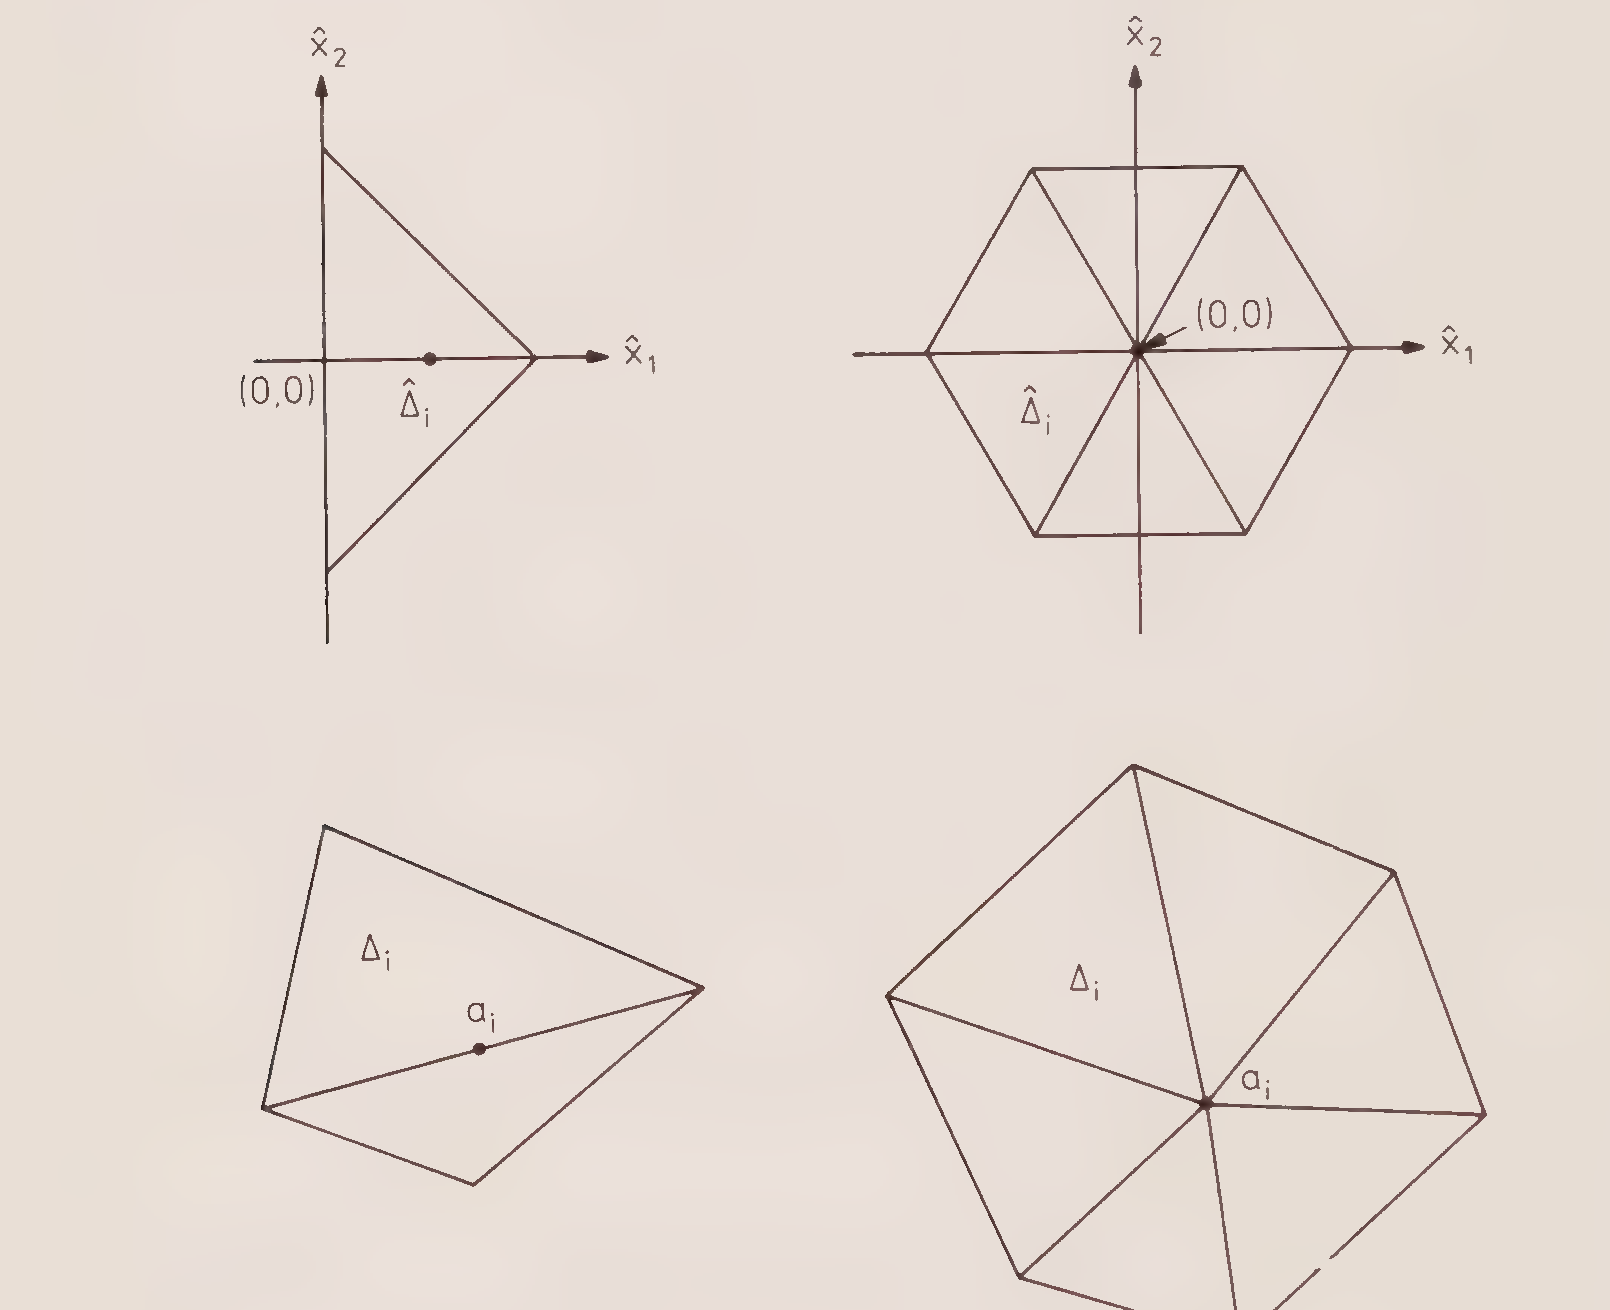
\includegraphics[width=.72\linewidth]{figures/appendix-figure-6.png}
\caption{区域 $\Delta_i$ 及其参考区域 $\hat\Delta_i$ 的例子.}
\label{fig:appendix-macroelements-reference-regions}
\end{figure}

现在可以利用局部 $L^2$ 投影定义插值算子
$R_h\in\mathcal{L}(L^1(\Omega);\Theta_h)$.
任取宏单元 $\Delta_i$, 记其参考区域为 $\hat\Delta_i$,
并取 $\hat v\in L^1(\hat\Delta_i)$.
令 $\hat R_i\hat v$ 是由
\begin{equation}\label{eq:appendix-local-regularization-projection}
\int_{\hat\Delta_i}
(\hat R_i\hat v-\hat v)p\,\mathrm{d}\hat x
=0
\qquad
\forall p\in P_k(\hat\Delta_i)
\end{equation}
确定的 $P_k(\hat\Delta_i)$ 中的唯一多项式.
对 $v\in L^1(\Omega)$, 定义 $R_hv\in\Theta_h$ 为
\begin{equation}\label{eq:appendix-local-regularization-interpolant}
R_hv
=
\sum_{i=1}^{N_h}
\hat R_i(v\circ F_{\Delta_i})(\hat a_i)\theta_i,
\end{equation}
其中 $\hat a_i=F_{\Delta_i}^{-1}(a_i)$.
Clément [21] 和 Bernardi (同前引文) 证明了该算子 $R_h$
基本上具有与 $I_h$ 和 $\widetilde I_h$ 相同的插值性质,
其优点是可以作用于粗糙函数. 主要的局部插值结果如下.

\MathBookSourcePage{125}
\setcounter{statement}{3}
\begin{Theorem}\label{thm:appendix-local-regularization-error}
设 $\mathcal{T}_h$ 是 $\Omega$ 的一个正则三角剖分,
$\kappa$ 是 $\mathcal{T}_h$ 的任意三角形,
$l$ 和 $m$ 是两个正整数, 其中 $0\leq l\leq k+1$,
$p$ 和 $q$ 是 $[1,\infty]$ 中的两个实数, 且
\[
W^{l,p}(\kappa)\hookrightarrow W^{m,q}(\kappa).
\]
记 $\Delta$ 为所有包含 $\kappa$ 的宏单元 $\Delta_i$ 之并.
则对所有 $v\in W^{l,p}(\Delta)$ 有估计
\begin{equation}\label{eq:appendix-local-regularization-error}
\|v-R_hv\|_{m,q,\kappa}
\leq
Ch_\kappa^{l-m+2(1/q-1/p)}
\|v\|_{l,p,\Delta},
\end{equation}
其中常数 $C$ 与 $\kappa$, $h$ 和 $v$ 无关.
\end{Theorem}
